\part{Développer une application en Python pour évaluer les modèles HTR}\label{partie_3}

La deuxième partie du stage était axée sur le développement applicatif. Dans le cadre de l'entraînement des modèles de segmentation et de transcription pour Lectaurep, ALMAnaCH. 

On souhaitait disposer d'un outil permettant de visualiser rapidement des informations sur la qualité des modèles de transcription et de segmentation, entraînés avec Kraken. 

Cependant, l'outil devait être suffisamment généralisable pour être réutilisé dans d'autres projets. L'application Kraken-Benchmark, créée durant mon stage, a permis de réaliser en partie ces objectifs.\footnote{La seconde mission de stage a été présentée sous la forme d'une \textit{issue} GitLab accessible via le lien : \url{https://gitlab.inria.fr/dh-projects/kraken-benchmark/-/issues/1}}.\\ 
\clearpage
\thispagestyle{empty}
\chapter{État de l'art pour l'évaluation des modèles de transcription entraînés avec le système HTR Kraken}

\section{Banc d'essai des outils existants : limites et avantages}

Dans de nombreux projet de recherche et de développement d'outils informatiques, on démarre rarement d'une simple page blanche. Avant de me pencher directement sur les aspects de développement et de gestion du projet, j'ai cherché à faire le bilan des solutions qui existait pour Lectaurep.\\

Lorsque Lectaurep utilisait encore Transkribus, les résultats étaient obtenus au cours d'une longue procédure. Une fois que le nombre de pages transcrites était suffisant, un mail était envoyé aux membres de l'équipe Transkribus pour leur signaler qu'ils pouvaient entraîner le modèle. Une fois cette tâche réalisée, ils répondaient en renvoyant un rapport contenant le taux d'erreur par caractères (\textit{Character Error Rate} ou CER) et le taux d'erreur par mots(\textit{Word Error Rate} ou WER) plusieurs jours après. Nous reviendrons sur la définition de ces métriques dans la section suivante. Étaient également joint à ces données, les deux versions du texte mises en vis-à-vis, comprenant le document de vérité terrain transcrit manuellement et la prédiction obtenue par le modèle\footnote{\cite{bonhomme_defis_2018}, pp. 41}.

Kraken est l'outil privilégié pour l'entraînement des modèles de segmentation et de transcription ainsi que pour effectuer des prédictions à partir des modèles. Cependant concernant, l'étape d'évaluation de la transcription obtenue, l'affichage dans le terminal ne permet pas de bien discerner les erreurs, du moins de bien les localiser.

\begin{wrapfigure}[18]{l}{10cm}
    \centering
    \centerline{\fbox{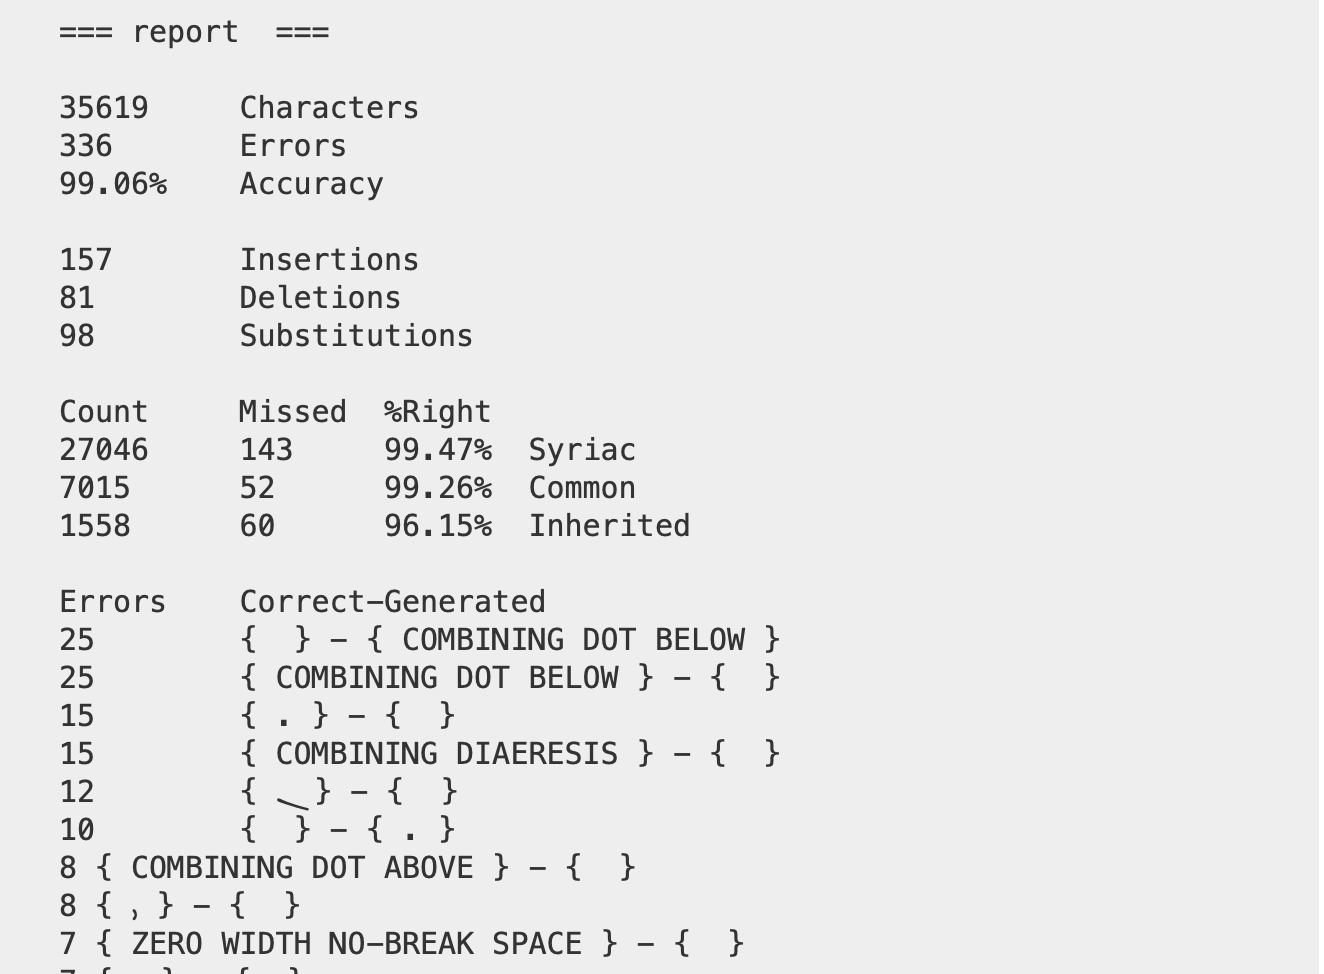
\includegraphics[width=10cm]{images_partie_3/rapport_kraken.png}}}
    \caption{Exemple de rapport fourni par kraken \textcopyright 2015, \cite{noauthor_kraken_nodate}}
    \label{fig:rapport_Kraken}
\end{wrapfigure} 

En effet, le rapport d'évaluation (Cf. Figure \ref{fig:rapport_Kraken}) de la transcription s'obtient grâce à la commande \citecode{\$ ketos test -m model images} et permet d'obtenir le nombre de caractère total dans la vérité terrain (sans donner le nombre de caractère total dans la prédiction), un taux de réussite général qui correspond au CER, le nombre d'insertions, de suppressions et de substitutions de caractères d'une version du texte à l'autre ainsi qu'une liste des erreurs les plus fréquentes (c'est-à-dire les pairs de caractères les plus confondues).\\

J'ai également voulu vérifier si d'autres outils d'évaluation de la sorte existaient déjà en parcourant les dépôts de code sur Github. J'ai donc relevé trois outils parmi lesquels :  Werpp\footnote{wer++, URL : \url{https://github.com/nsmartinez/WERpp}}, XER\footnote{xer, URL : \url{https://https://github.com/jpuigcerver/xer}} et WER-in-python\footnote{WER-in-python, URL : \url{https://github.com/zszyellow/WER-in-python}} à partir de deux fichiers texte d'exemples comprenant 10 à 20 mots. Le premier représentant un document de vérité terrain, l'autre étant censé montrer la transcription avec des erreurs volontairement insérées (omission de la ponctuation, ajout de majuscules ou de minuscules indésirables, espaces conséquences entre certains mots etc.).\\

Une fois les tests effectués, j'ai pu relever les points suivants :
\begin{itemize}
    \item Certains programmes n'utilisaient pas les mêmes versions de Python, comme Werpp qui présentait des défauts de compatibilité avec la version 3. Pour le faire fonctionner, il a fallu modifier quelques lignes de codes afin de le rendre exécutable;
    \item Certaines options proposées par ces programmes comme dans Werpp ou XER ne fonctionnaient pas. Ainsi dans le cas de XER le chargement des fichiers au format texte ne fonctionnait pas. Il fallait inscrire les phrases dans le terminal avec une commande du type \citecode{\$ xer -i str -r "Je suis un document valide" -t "je suis Unn DoCument, invalide !"} ce qui n'est évidemment pas du tout envisageable pour des transcriptions de plus de 10 lignes de texte. D'autres, options comme la colorisation des résultats pour les lettres manquantes, proposé par Werpp, ne fonctionnaient pas en raison d'un problème de spécification des \textit{packages} requis;
    \item Certains outils ne permettaient pas de cumuler en sortie plusieurs résultats en même temps comme le WER et le CER. C'est par exemple le cas de WER-in-python et Werpp;
    \item Enfin les temps de calculs pouvaient s'avérer très longs et la plupart des codes n'étaient pas bien documentés, l'usage des commandes devant être déduites de la lecture du code.\\
\end{itemize}
\medskip
Si la plupart de ces outils ne se sont pas révélés directement utilisables pour notre projet, ce premier état de l'art m'a permis de me poser les questions quant aux fonctionnalités qui pouvaient être réutilisées et aux métriques qui pourraient s'avérer utiles dans la future application. 

De plus la lecture du code, m'a permis de me familiariser avec la création de CLI par le biais du \textit{package} intégré à Python \textit{argparse}. 

\textit{Argparse} est un \textit{package} Python permettant d'écrire rapidement des programmes sous forme de CLI en récupérant un ensemble de fonctions réutilisables pour permettre entre autre la gestion des arguments entrés par l'utilisateur dans le terminal, la documentation, etc.\\

Afin de me familiariser avec les logiques de fonctionnement du CLI, j'ai créé un premier programme \citecode{cerwer\_tool}\footnote{Le dépôt du code de l'outil \citecode{cerwer\_tool.py} est disponible sur Github, URL : \url{https://github.com/Lucaterre/cerwer_tool}} en adaptant certaines fonctions des outils décrits plus haut, qui allaient préfigurer le développement de l'outil Kraken-Benchmark spécifique au projet.\\

L'outil \citecode{cerwer\_tool.py} permettait, en outre, au moyen d'une ligne de commande prenant en argument deux fichiers texte correspondant à une vérité terrain et une prédiction, d'émettre un rapport dans le terminal comportant le nom de l'utilisateur, le texte de référence, le texte prédit, de comparer le nombre de mots et de lettres insérées, substituées et supprimées et enfin d'afficher le WER et le CER.

L'utilisateur avait la possibilité de sauvegarder le rapport dans un fichier texte pour garder une trace et de produire un graphique présentant le nombre d'insertions, substitutions et de suppressions sur le nombre de mots total (Cf. Figure \ref{fig:cerwer}).\\
\newpage
Cependant cet outil avait des limites : il supposait de récupérer en amont la transcription HTR, avec Kraken, dans un fichier texte pour utiliser \citecode{cerwer\_tool.py}. Comme nous le verrons par la suite, nous avons intégré cette chaîne de traitement HTR directement dans l'outil Kraken-Benchmark en réutilisant le code de Kraken par l'intermédiaire de son API.

\begin{figure}[h]
    \centering
    \centerline{\fbox{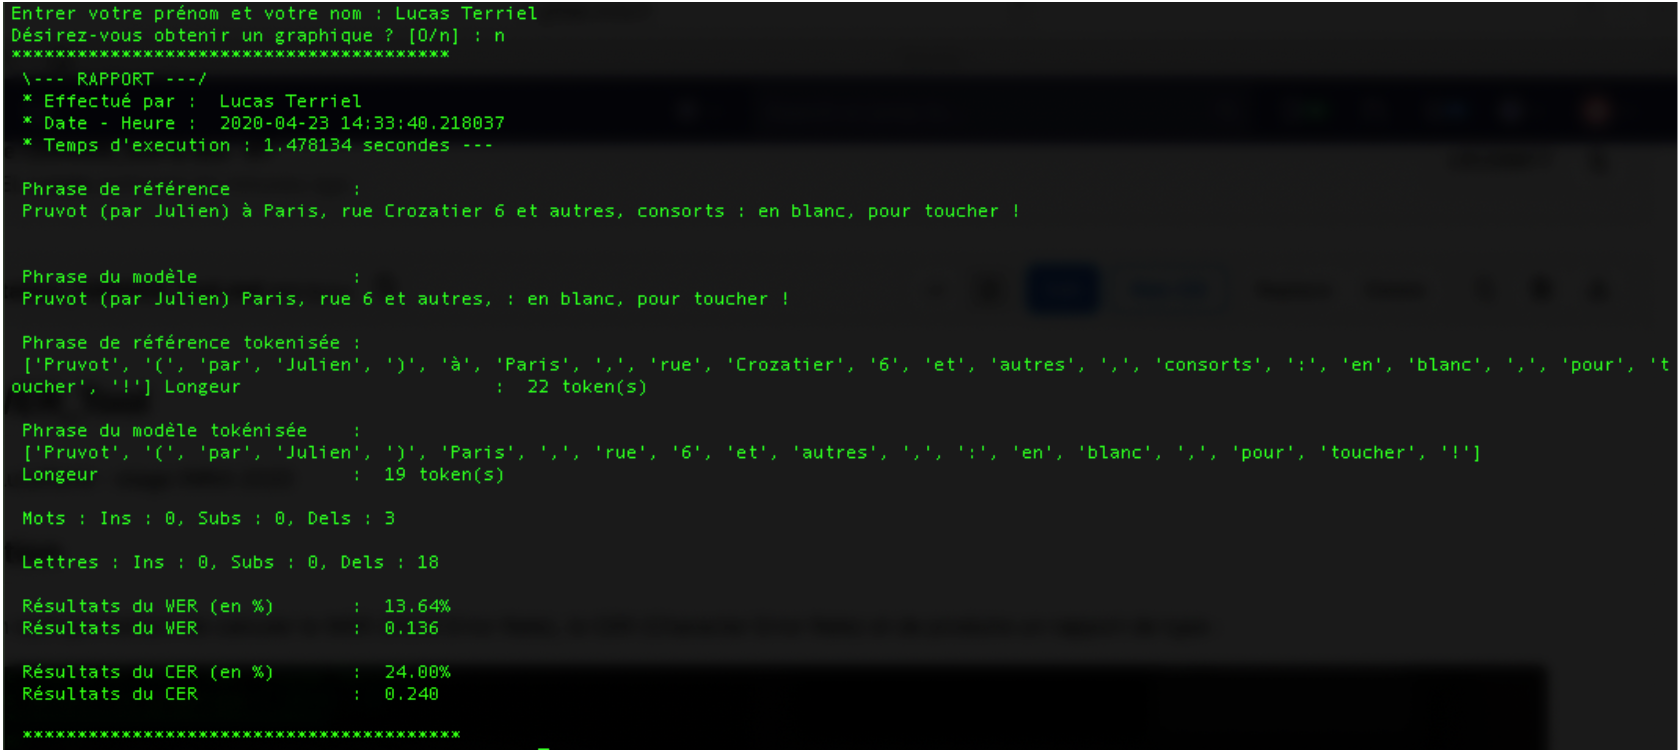
\includegraphics[width=18cm]{images_partie_3/cerwer_tool.png}}}
    \caption{Capture d'écran du rapport produit par le prototype \citecode{cerwer\_tool.py} \textcopyright L. Terriel, 2020, \textit{Pycharm}}
    \label{fig:cerwer}
\end{figure}
\newpage
\section{Des métriques pour comparer la transcription HTR et la vérité terrain}\label{metriques}

Après avoir formulé un état de l'art, je me suis penché sur les méthodes de calcul qui permettent d'évaluer une transcription HTR avec sa vérité terrain. C'est un problème qui peut être ramené à la comparaison de deux chaînes de caractères entres-elles (comparaison \textit{text-to-text}). Dans un deuxième temps, pour permettre d'évaluer les transcriptions dans un contexte de traitement par le TAL, je me suis également intéressé aux métriques permettant d'apprécier la proximité sémantique entre des mots appartenant à deux documents différents.\\

J'ai exposé et synthétisé ce travail de recherche dans un \textit{notebook} Jupyter. Un \textit{notebook} peut être conçu comme un calepin électronique qui permet d'écrire du texte brut et du code dans un même temps. Comme nous le verrons par la suite, il est indispensable dans tout travaux concernant le traitement de données en ML et DL, notamment pour expérimenter des calculs et des scripts de code.\footnote{Le \textit{notebook} de recherche est disponible dans plusieurs formats dans les Annexes \citecode{/C-Application\_Kraken\_Benchmark/Documentation-Reasearch/\\Evaluation de la similarité entre deux séquences dans le contexte de la reconnaissance automatique de caractère} }. Le \textit{notebook} résume brièvement les définitions et usages des métriques, les visualisations possibles à partir de ces dernières et les différents algorithmes qui permettent de les implémenter dans un programme.\\

\subsection{La comparaison de chaînes de caractères}

Parmi les métriques et les algorithmes associés qui permettent d'évaluer la similarité entre deux phrases (similarité syntaxique) :\\

\textbf{Le similarité Ratcliff/Obershelp -} L'algorithme de Ratcliff/Obershelp (ou \textit{Gestalt Pattern Matching}) se base sur la recherche de sous-chaînes de caractères communes (\textit{subpattern}) entre deux séquences de caractères.\\

Le principe de l'algorithme de Ratcliff/Obershelp repose sur une découpe des phrases en deux parties en se plaçant par rapport à une ancre qui correspond au premier point de différentiation entre les deux séquences. De part et d'autre, le processus itératif évalue à gauche puis à droite des séquences les plus longues les sous-chaînes communes, jusqu'à ce que la longueur des séquences soit intégralement parcourue.\\
\newpage
La similarité Ratcliff/Obershelp ($ Similarite_{RO} $) calcule deux fois le nombre de caractères effectivement reconnus ($Sub_{caracteres}$) dans les sous-chaînes les plus longues ($\, 2 \cdot Sub_{caracteres} \,$) sur le nombre total de caractères compris dans les deux phrases.\\

soit : $$ Similarite_{RO} = \frac{2Sub_{caracteres}}{|Chaine_1|+|Chaine_2|} $$

où : $$ 0 <= Similarite_{RO} <= 1 $$

Par exemple, soit $ S_1 \,= $ \inquote{J'AIME LE CHOCOLAT} et $ S_2 \,=$ \inquote{J'AIME LA CHOCOLATINE}\\

pour $$Similarite_{RO}(S_1 \,, S_2 \,) = \frac{2 \, \times \, ([J'AIME\, L\,] + [\, CHOCOLAT])}{|S_1|+|S_2|} = \frac{34}{39} \simeq  \, 0,87$$\\ 

Dans cet exemple, l'algorithme de Ratcliff/Obershelp trouve dans un premier temps \inquote{J'AIME L} à gauche comme la plus longue sous-chaîne commune puis à droite \inquote{ CHOCOLAT} (espace compris).\\

Pour inclure ces métriques dans un programme informatique le \textit{package} Python \textit{difflib} permet de récupérer des fonctions qui se base sur cet algorithme.\\

L'avantage de cet algorithme est qu'il permet d'obtenir un score rapidement afin de comparer deux chaînes de caractères. Cependant elles ne rendent pas compte précisément des modifications de caractères qui ont pu s'opérer lors du passage d'une chaîne à une autre. Nous allons voir en quoi les distances mathématiques peuvent nous y aider.\\

\textbf{Les distances de Levensthein, de Hamming et de Damerau-Levenshtein -} La distance de Levensthein\footnote{Établie en 1965 par le mathématicien russe Vladimir Levenshtein (1935-2017)} (encore appelé distance d'édition), est une distance mathématique, et une généralisation de la distance de Hamming, dans le sens où la première peut travailler sur des chaînes de longueur, ce n'est pas le cas pour la seconde.\\

La distance de Levensthein évalue le coût minimal de transformation d'une de caractère $R$ en une chaîne de caractère $P$ en effectuant les opérations suivantes auxquelles sont associés un coût de 1:

\begin{itemize}
    \item La \textbf{substitution} d'un caractère de $R$ par un caractère de $P$;
    \item L'\textbf{insertion} d'un caractère dans $R$ par $P$;
    \item La \textbf{suppression} d'un caractère dans $R$ par $P$;
\end{itemize}

Pour illustrer le calcul de cette distance nous pouvons prendre les exemples suivants :

\begin{itemize}
    \item soit $R = magasin$ et $P= magasin$, alors $LD(R, P) = 0$, car il n'y a pas de changement.
    \item soit $R = magasin$ et $P= megasinier $, alors $LD(R, P) = 4$, car il eu 3 insertions \inquote{ier} et une substitution \inquote{a} en \inquote{e}. 
\end{itemize} 
\bigskip
La distance de Damerau-Levenshtein\footnote{\cite{chaumartin_traitement_2020}, pp. 132} est une variation de la distance de Levensthein qui inclut les transpositions dans les opérations (pour prendre en compte les fautes d'orthographe ou les échanges de caractères).\\ 

Par exemple dans le cas des mots \inquote{acceuil}, \inquote{auteuil} et \inquote{accueil}, la distance de Levensthein calcule une distance de 2 entre chaque mots. Cependant \inquote{acceuil} et \inquote{accueil} sont plus proches (transposition de \inquote{eu} en \inquote{ue}) que \inquote{auteuil} et \inquote{acceuil}, la distance de Damerau-Levenshtein prend en compte cette différence. Ainsi \inquote{acceuil} et \inquote{accueil} vaudront 1 tandis que \inquote{auteuil} et \inquote{acceuil} vaudront 2 une transposition de caractères coûte moins qu'une substitution de caractères. 

Cette distance est plutôt utilisée dans le cadre de correcteur orthographique, de plus la complexité algorithmique de la distance de Damerau-Levenshtein est plus élevée que la distance de Levensthein, ce qui est une caractéristique à prendre compte durant l'implémentation. La distance de Damerau-Levenshtein sera plus longue à calculer que la distance de Levensthein (environ 20 secondes pour la première et 0.01 secondes pour la seconde (implémentation la plus rapide) pour des chaînes d'environ 350 caractères).\\

Il existe plusieurs algorithmes pour implémenter cette distance\footnote{\cite{noauthor_algorithm_nodate}}, mais la tâche peut être facilité par des \textit{packages} en Python, comme la fonction \citecode{\_fast\_levenshtein()} de l'API de l'\textit{Kraken}\footnote{\cite{noauthor_kraken_nodate}} ou encore  \textit{python-levenshtein}\footnote{\cite{noauthor_python-levenshtein_nodate}} qui est une implantation plus rapide de la distance (extension écrite en langage C).\\

Nous allons voir que cette distance est importante si on veut pouvoir calculer le taux d'erreur par caractères (CER) et le taux d'erreur par mots (WER).\\ 

\textbf{Le taux d'erreur par caractères et le taux d'erreur par mots -} Le taux d'erreur par caractère (\textit{Character error rate} ou CER) et le taux d'erreur par mots (\textit{Word error rate} ou WER) sont des taux d'erreurs très utilisés pour constater l'efficacité d'un modèle de reconnaissance. Le CER et le WER se calcule de la manière suivante :

Si : 

\begin{itemize}
    \item $N$ est le nombre total de caractères ou de mots contenus dans la phrase de référence;
    \item $S$ (\textit{Substitution}) est le nombre de substitutions (mots ou caractères incorrectement reconnus);
    \item $D$ (\textit{Deletion}) est le nombre de suppressions (mots ou caractères omis);
    \item $I$ (\textit{Insertion}) est le nombre d'insertions (mots ajoutés).
\end{itemize}

Le CER se calcule tel que : $$ Character\, Error\, Rate = \frac{S\, + \,D\, + \,I\,}{N_{total\, de\, caracteres}} $$

Le WER se calcule tel que : $$ Word\, Error\, Rate = \frac{S\, + \,D\, + \,I\,}{N_{total\, de\, mots}} $$

Dès lors si on connaît la distance de Levensthein $D$ pour une phrase de référence notée $R$ et une phrase de prédiction $H$, le CER peut être ramené à l'expression suivante : $$CER = \frac{D(R,H)}{N_{total\, de\, caractères}}$$  et le WER :$$WER = \frac{D(R,H)}{N_{total\, de\, mots}}$$\\

Les résultats obtenus sont interprétés de la sorte : plus le taux approche 0 plus la reconnaissance est efficace, à l'inverse, plus le taux se rapproche de 1, plus le texte à eu du mal a être reconnu. Il peux même dépasser 1, si la reconnaissance est très mauvaise, surtout s'il y a eu beaucoup d'insertions. Nous avons été confronté à ce cas comme nous le verrons en chapitre \ref{tests_KB_lectaurep}.\\
\newpage
A partir du WER on peut également calculé le taux de reconnaissances de mots (ou \textit{Word Accuracy} (WAcc)) calculé de la manière suivante, pour obtenir un pourcentage (à noter que le résultat peut-être négatif si le WER dépasse 1): $$W_{ACC}\, = (1 - WER) \cdot 100  $$

Le CER est plus significatif que le WER et le taux de reconnaissance par mots dans le sens où ces derniers sont corrélés aux erreurs de prédiction des caractères effectués par le modèle, \textit{de facto} le WER augmente et le le taux de reconnaissance par mots baisse quand le CER augmente.

\subsection{Estimer la similarité entre deux documents}

L'intuition est de prendre la vérité terrain comme premier document et sa prédiction par le modèle HTR comme un deuxième document. L'indice de Jaccard ainsi que la similarité cosinus peuvent nous y aider :\\

\textbf{L'indice de Jaccard -} Son but est d'estimer le pourcentage de mots communs aux deux documents. L'indice évalue, sur l'union de deux ensembles (deux phrases par exemple), la taille de l'intersection qui regroupe les mots en commun dans la transcription de référence et dans la transcription HTR, divisée par la taille de l'union de deux ensembles.

Il est formulé comme suit : $$ J(doc_1,doc_2) = \frac{|doc_1 \cap doc_2|}{|doc_1 \cup doc_2|} $$

Plus le résultat approche de 1, plus les documents sont similaires, car le nombre des mots partagés par la référence et par sa transcription HTR dans l'intersection est important. À l'inverse, si le résultat est plus proche de 0, alors on peut en conclure que les deux textes sont davantage éloignés l'un de l'autre.\\

\textbf{La similarité cosinus -} Si l'on reprend la Figure \ref{fig:word_embedding} de la section \ref{TAL_repertoire}, il s'agit de calculer l'angle cosinus noté $cos(\theta)$ entre des mots, alors représentés sous la forme de vecteurs, afin de mesurer leur degré de proximité. La formule de la similarité cosinus est la suivante : $$ similarite\, cosinus \, = cos\, (\theta\,) = \frac{\overrightarrow{V1}\, \times \,\overrightarrow{V2}}{||\overrightarrow{V1}||\, \times \,||\overrightarrow{V2}||} $$

où : 

$$ ||\overrightarrow{V1}||\, et\, ||\overrightarrow{V2}||\, >\, 0 $$

Les résultats obtenus sont interprétés de la manière suivante, en fonction de la valeur de $cos(\theta)$ :

\begin{itemize}
    \item Plus elle tend vers 0, plus les vecteurs sont dits indépendants ou opposés (orthogonaux) : les documents sont donc éloignés;
    \item Plus elle tend vers 1, plus les vecteurs sont dits (colinéaires de coefficient positif) donc les documents sont proches;
\end{itemize}

\subsection{Remarques complémentaires sur les métriques d'évaluation utilisées}

Nous avons présenté les principales métriques que nous retrouverons dans l'application Kraken-Benchmark. La première catégorie de métrique prenant en compte la place du mot et du caractère dans les séquences, la deuxième cherchant à rassembler les mots pour évaluer leur proximité sémantique.\\

Il faut noter que pour permettre l'implémentation de ces métriques dans un programme informatique des étapes de normalisation des données textuelles sont requises : on parle de \textit{data pre-processing}. 

Ces méthodes sont empruntées aux tâches du TAL déjà présentées en section \ref{TAL_repertoire}. Ainsi pour calculer la distance de Levensthein, le CER et le WER, on pourra avoir recours à un découpage des phrases en caractères ou en mots (\textit{tokenisation}). 

Pour la similarité cosinus, en plus du découpage en mot, on peut avoir recours à une suppression des mots les plus fréquents (\textit{stops words}), ainsi qu'au plongement des mots pour les convertir en valeurs numériques (\textit{word embedding}) afin de représenter sous la forme vecteurs.\\

Pour terminer, en vue de ne pas surcharger le présent mémoire de code brut, il est possible de retrouver dans le \textit{notebook} intitulé \inquote{Évaluation de la similarité entre deux séquences dans le contexte de la reconnaissance automatique de caractères} davantage de précisions sur les métriques, les étapes de normalisation du texte, leurs différentes implémentations en Python, des tests de durée d'exécution et les visualisations rendues possibles (graphiques, matrices de confusion etc.).\\

\chapter{Le développement d'une application : Kraken-Benchmark}

\section{Modélisation}

\subsection{Les objectifs fixés au début du développement}\label{objectifs}
En concertation avec ma tutrice de stage, Alix Chagué, j'ai fixé des cas d'usages (\textit{use case}) et formaliser les objectifs idéaux à atteindre dans la conception de l'application. Ceci dans l'optique de  décrire les exigences fonctionnelles de la future application. Nous avons donc relevé que :

\begin{itemize}
    \item L'application doit pouvoir comparer et évaluer la qualité d'un modèle de transcription et/ou de segmentation à l'échelle d'une ou de plusieurs images;
    \item Les résultats de l'évaluation doivent être accessibles et visualisables dans une interface conviviale pour l'utilisateur (\textit{user-friendly});
    \item Le rapport produit doit pouvoir être exporté dans plusieurs formats;
    \item L'utilisateur doit avoir la possibilité de charger les images et le modèle facilement;
    \item Le programme doit être écrit en Python 3 pour assurer sa  maintenabilité dans le temps;
    \item Le code, et l'application, doivent disposer d'une documentation interne et externe;
    \item Le programme doit pouvoir être généralisé à d'autres projets et/ou viser une interropérabilité avec la plate-forme eScriptorium à terme;
\end{itemize}

Nous verrons dans la section \ref{perspectives_amélios} quels objectifs ont été atteints, ceux qui restent en cours de développement et ceux qui ont émergés au cours des tests et rédaction du code. 

\subsection{Un écosystème Python orienté pour la science des données et la conception d'application web}

Pour réaliser l'application Kraken-Benchmark en Python (l'ensemble des fichiers de l'application cités à partir de maintenant sont disponibles dans les Annexes C), il m'a fallut disposer de solutions pour concevoir l'interface, mais aussi pour réaliser des tâches plus précises comme les calculs et les représentations graphiques de données (\textit{data visualisation}). Quand il s'agit d'évaluer des données, Python fait graviter autour de lui un ensemble d'outils orientés pour la science des données (\textit{data science}, Cf. Figure \ref{fig:eco_datascience}).

On peut concevoir ce vaste écosystème comme une boîte à outils qui permet de réaliser des tâches précises, notamment pour comparer des données entre elles.  

\begin{figure}[h!]
    \centering
    \centerline{\fbox{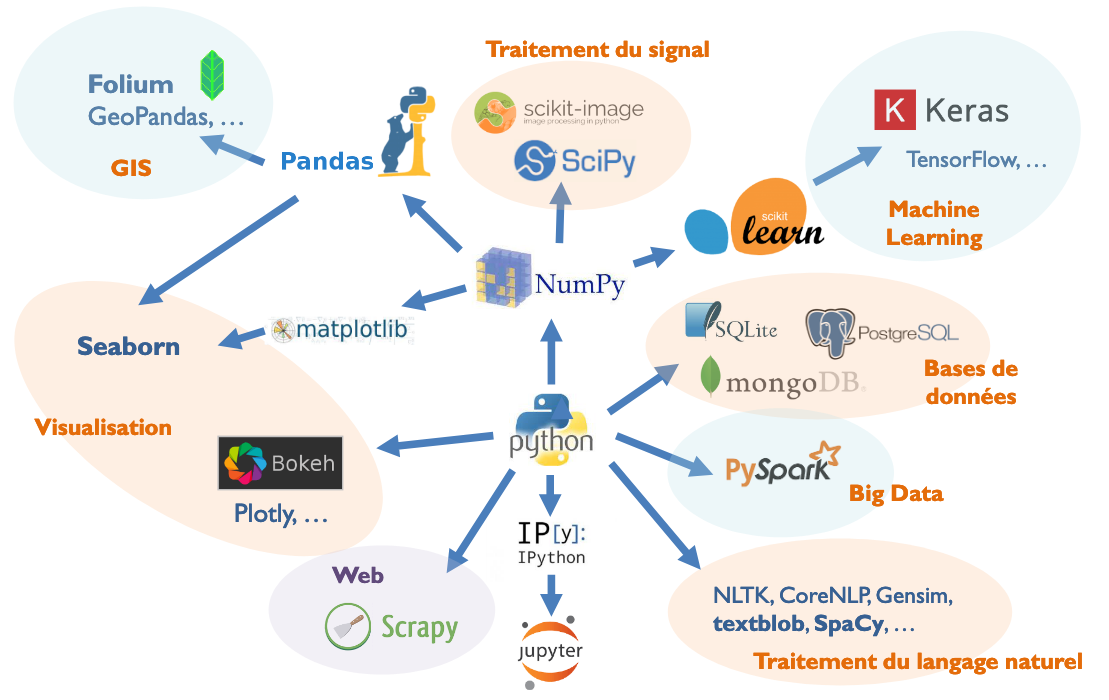
\includegraphics[width=15cm]{images_partie_3/ecosysteme_datascience.png}}}
    \caption{L'écosystème Python pour la science des données (\textit{datascience})   \textcopyright F.Pennerath, Mineure \inquote{Data Science}, Centrale Supélec}
    \label{fig:eco_datascience}
\end{figure}

Dès lors, l'application Kraken-Benchmark requiert pour fonctionner, outre le langage Python 3, l'installation des \textit{packages} suivants (certains ont déjà étaient aperçus dans les sections précédentes et d'autres étant déjà inclus dans le langage Python) : 

\begin{itemize}
    \item Pour réaliser les calculs et l'implémentation des \textbf{métriques d'évaluation} : Sklearn\footnote{\cite{noauthor_scikit-learn_nodate}}, Numpy\footnote{\cite{noauthor_numpy_nodate}}, Python-Levenshtein\footnote{\cite{noauthor_python-levenshtein_nodate}}, Kraken API\footnote{\cite{noauthor_kraken_nodate}}, difflib, math, collections;
    \item Pour réaliser les \textbf{visualisations de données} : Matplotlib\footnote{\cite{noauthor_matplotlib_nodate}}, Seaborn\footnote{\cite{noauthor_seaborn_nodate}}, Pandas\footnote{\cite{noauthor_pandas_nodate}};
    \item Pour le \textbf{pré-traitement des données textuelles} (découpage des phrases en mots et suppressions des mots les plus fréquents) : NLTK\footnote{\cite{noauthor_nltk_nodate}}
\end{itemize}

À coté de ses \textit{packages} orientés science des données, j'ai eu besoin de recourir à des \textit{packages} plus spécifiques : 

\begin{itemize}
    \item Traitement des images en entrée : Pillow\footnote{\cite{noauthor_pillow_nodate}};
    \item Réalisation de la chaine de traitement HTR : Kraken API;
    \item Gestion de la partie CLI : argparse;
    \item Gestion de la partie GUI (\textit{Graphical User Interface}) de l'application dans le navigateur \textit{web} : Flask\footnote{\cite{noauthor_flask_nodate}}
\end{itemize}

Initialement au début du projet il était prévu de n'utiliser que le moteur de \textit{templates}\footnote{Un moteur de \textit{templates} permet de séparer la partie traitement pur des données en Python de la partie visuelle de l'application. Le \textit{template} d'un projet \textit{web} contiendra tous les fichiers HTML (pour la structure), le CSS et les images (style et aspect visuel du site), et le Javascript (pour les animations).} \textbf{Jinja}\footnote{cite package}. Cependant, j'ai rapidement constaté les limites, notamment quand je devais permettre à l'utilisateur de pouvoir accéder à plusieurs pages dans le navigateur (plusieurs vues), un gestionnaire de \textit{templates} seul n'était pas suffisant. 

L'avantage de \textbf{Flask} repose sur le fait qu'il s'agit d'une boîte à outils (mini \textit{framework} \textit{web}) pour construire des applications \textit{web}. Ainsi en plus d'intégrer le moteur de \textit{templates} \textbf{Jinja}, il intègre un gestionnaire de routes (les différentes routes URL pour définir les vues), et dispose d'un gestionnaire de requêtes HTTP ainsi que d'un serveur de développement\footnote{On distingue le serveur de développement, pour tester les applications \textit{web}, du serveur de production, qui permet de déployer et d'installer l'application \textit{web} finalisée qui est donc accessible aux utilisateurs.} pour tester l'application\footnote{\textbf{HTTP} (HyperText Transfer Protocol), est un protocole de communication entre client et serveur pour le \textit{web}.} et pour communiquer avec le code Python (ou WSGI\footnote{WSGI ou \textit{Web Server Gateway Interface}, est interface entre des serveurs et des applications \textit{web} pour Python. c'est une spécification qui permet à l'application Python de recevoir une requête HTTP transformée en un objet Python et de retourner une réponse HTTP sous la forme d’un autre objet Python également.}) \textbf{Werkzeug}\footnote{cite package}.\\

La plupart des \textit{packages} Python listés ci-dessus sont disponibles avec la distribution Python \textbf{Anaconda}. Il s'agit d'une distribution de Python comprenant le langage Python 3 mais également un ensemble de \textit{packages} dédiés à la science des données. Ainsi plutôt que de devoir installer les \textit{packages} un à un via le gestionnaire de base \textbf{pip}\footnote{\textbf{pip} est le gestionnaire de \textit{packages} Python par défaut. Il permet d'installer des \textit{packages} supplémentaires dans la distribution Python classique par l'intermédiaire d'une commande de type \citecode{pip install nom-du-paquet}.}, l'utilisateur pourra créer un environnement virtuel \textbf{conda} par le biais du fichier \citecode{environment.yml} qui regroupe les \textit{packages} cités plus haut.\\ 

L'installation et les commandes pour utiliser l'application sont résumés dans un fichier de type \inquote{lisez-moi} (\citecode{README.md}).

\subsection{Les étapes de fonctionnement : retour sur les aspects de programmation}

Après avoir rassemblé les outils pour réaliser le programme, j'ai modélisé les différentes étapes qu'il devait réaliser. De la même manière que pour développer l'outil \textit{Generator Lectaurep-TEI} abordé dans la section \ref{generator-lecto-dev}, j'ai créé un modèle résumant l'algorithme de l'application (Cf. Figure \ref{fig:algo-kb}).\\

Le programme se résume aux étapes suivantes :
\begin{enumerate}
    \item Avant de lancer le programme, l'utilisateur place dans différents dossiers les fichiers à traiter. 
    Placé à la racine du script principal \citecode{kraken\_benchmark.py} l'utilisateur peut créer le dossier \citecode{dataset\_GT} qui reçoit les fichiers en texte brut de la vérité terrain, le dossier \citecode{images} qui reçoit les images (format .jpeg) à reconnaître, et dans le dossier \citecode{model} un modèle (.mlmodel) pré-entraîné avec \textit{Kraken}. L'utilisateur doit conserver le même ordre de fichiers dans les dossiers \citecode{dataset\_GT} et \citecode{images} en utilisant un label dans les nommages de fichiers. Ainsi les images pourront être notés \citecode{image\_1, image\_2 etc.} et les transcriptions \citecode{transcription\_1, transcription\_2 etc.}. Sans cet étiquetage le programme risque d'associer une image avec la mauvaise transcription. Une fois cette étape réalisée, on peut lancer le programme via la commande \citecode{\$ python kraken\_benchmark.py}. L'utilisateur peut également spécifier des options derrière sa commande comme \citecode{- -label} s'il souhaite renseigner des métadonnées sur ces images, \citecode{- - verbosity} si l'utilisateur souhaite avoir un rapport complet durant chacune des étapes du programme, et une option \citecode{- - clean\_text} qui permet en outre d'enlever la ponctuation et les caractères non alphabétiques, ce qui peut-être utile pour certains types de projets.\\
    \item Le script principal \citecode{kraken\_benchmark.py} lance une première étape de transcription HTR (qui s'appuie sur les modules de l'API Kraken). Après avoir associés les images avec leur transcription vérité terrain, le programme effectue le processus suivant : il charge modèle transcription et les images, les images sont binarisées, il procède ensuite à la segmentation des images pour repérer les coordonnées, et effectue les prédictions qui sont normalisées dans un encodage Unicode;
    \item Le script principal \citecode{kraken\_benchmark.py} rassemble alors, par triplet : l'image, la vérité terrain et la prédiction;
    \item Chacun des triplets est alors transformé en objets \citecode{SynSemTS} appartenant au module \citecode{SynSemTS.py} sur lesquels ont peux récupérer les différentes métriques et visualisations associées;
    \item Le groupe d'objets est alors récupéré par le module \citecode{kb\_report} qui se charge d'ouvrir le navigateur \textit{web} automatiquement sur un serveur de développement par défaut;
    \item L'utilisateur peut alors circuler dans l'application et afficher les différentes pages web. Le script \citecode{routing.py} du dossier \citecode{kb\_report} est chargé d'envoyer et de recevoir les requêtes URL pour afficher la page HTML correspondante durant la navigation de l'utilisateur, jusqu'à la fin de la session.
\end{enumerate}
Dans les sections qui suivent nous avons souhaité relater quelques questions de programmation rencontrées au cours du développement de l'application, plutôt que de simplement montrer le code Python brut. 

Le code source de l'application est consultable dans l'Annexe C, et une documentation interne au code explicite le rôle de chaque fonctions codés sous la forme de \textit{docstrings}\footnote{Les \textit{docstrings} dans du code informatique sont des chaînes de texte situées à certains endroits visant à expliciter le rôle des fonctions et/ou des étapes du code, par exemple. Elles visent à rendre le code source plus compréhensible pour les personnes qui souhaiteraient le réutiliser ou le maintenir. Elles peuvent suivre des conventions comme la PEP 257, le modèle Sphinx, ou le style Google Python.}. 

\begin{figure}[H]
    \centering
    \centerline{\fbox{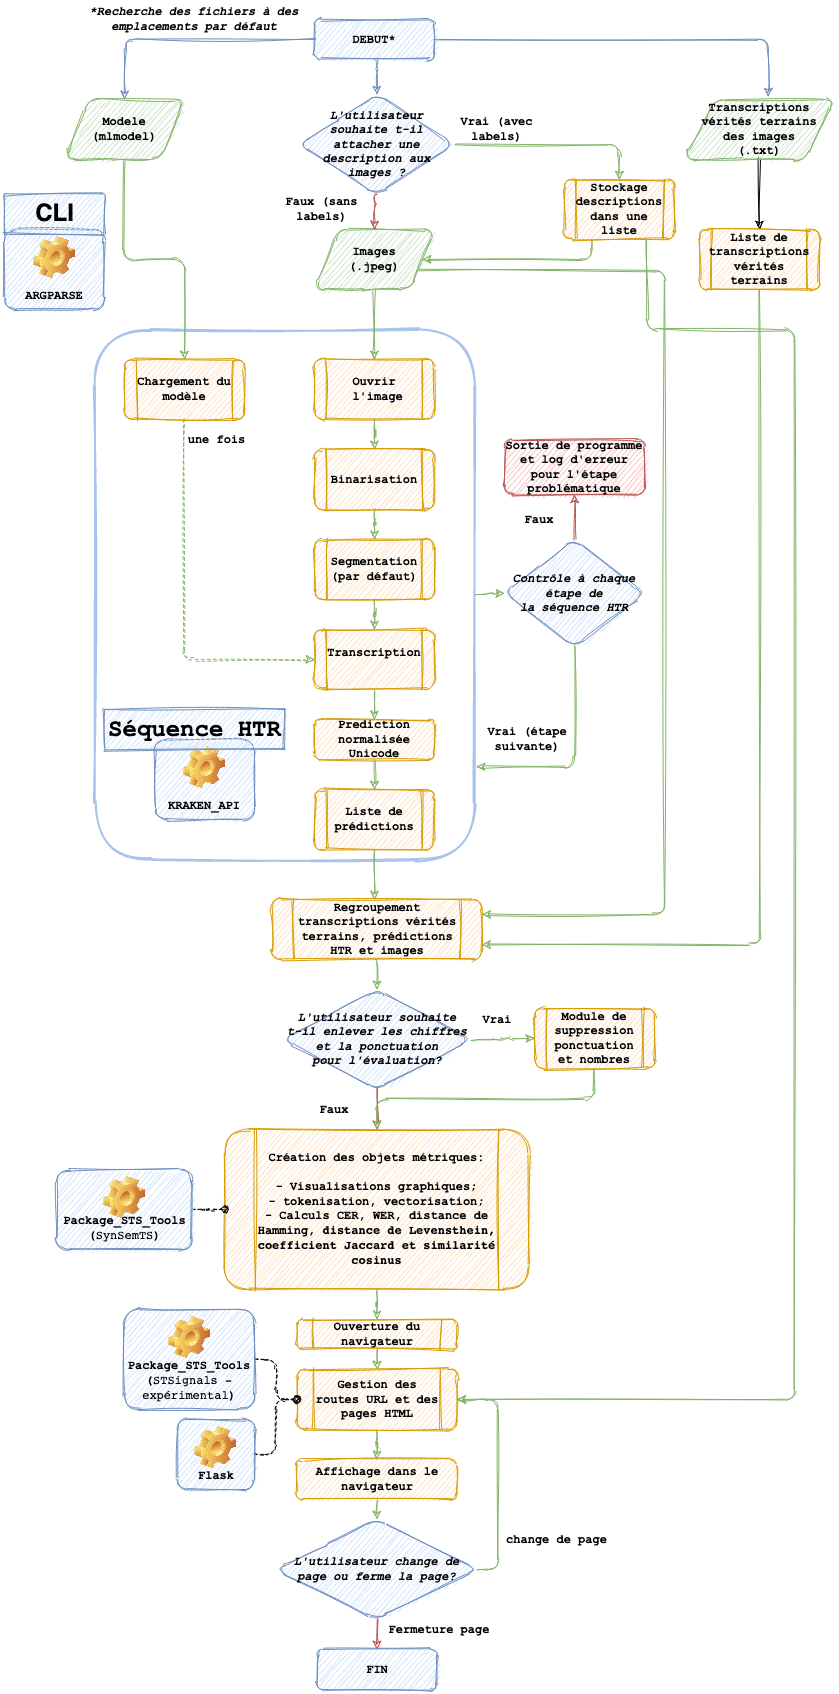
\includegraphics[width=17cm, height=22.5cm]{images_partie_3/Kraken-Benchmark_modelisation.png}}}
    \caption{Algorigramme de Kraken-Benchmark.   \textcopyright L. Terriel, 2020, Diagrams.net}
    \label{fig:algo-kb}
\end{figure}

\subsubsection{Un jeu de données pour tester l'application au cours du développement}

Durant le développement de l'application, je devais disposer de transcriptions de vérité terrain et d'un modèle de transcription. J'ai constitué un jeu de données en me basant sur des extraits de l'ouvrage \textit{Voyage au centre de la Terre} de Jules Verne (dossier \citecode{jules\_verne\_set\_test}).

Dans un premier temps, j'ai trouvé sur Gallica\footnote{Bibliothèque numérique de la Bibliothèque nationale de France} une série de 8 images hétérogènes. Parmi celles-ci, certaines contenaient du texte imprimé sur toute la page et d'autres des illustrations, de taille variable, dans l'optique de tester ces différences. 

La deuxième étape a été de constituer des vérités terrains en me basant sur l'environnement de transcription de Kraken (Cf. Figure \ref{fig:transcrire_kraken}). 

Après avoir lancé la ligne de commande correspondante, la transcription apparaît sur une page HTML qui comprend, à gauche l'image et à droite les lignes à transcrire. Cela peut s'apparenter à une version minimaliste de la plate-forme eScriptorium.   

\begin{figure}[h!]
    \centering
    \centerline{\fbox{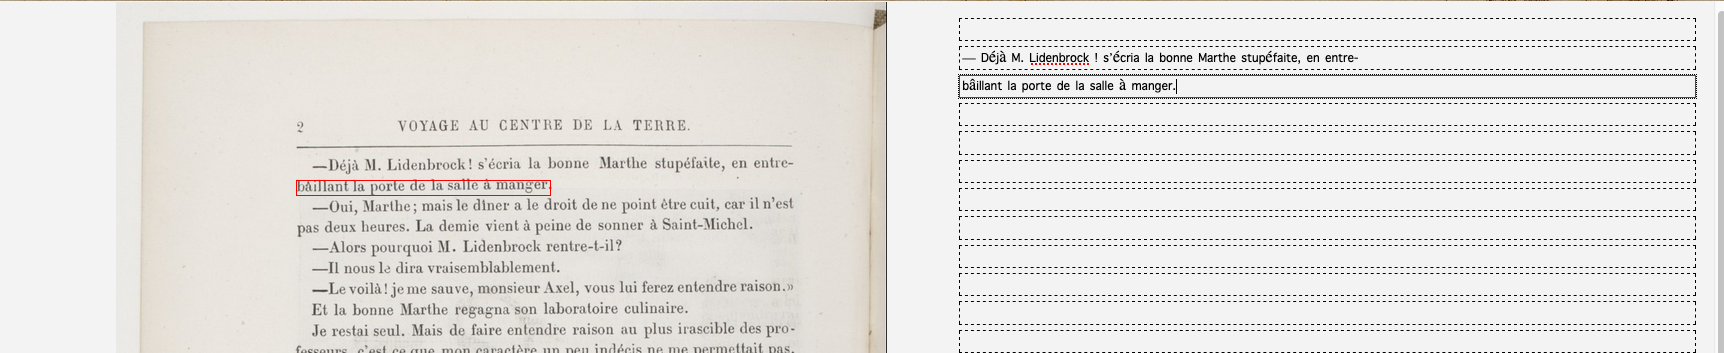
\includegraphics[width=19cm]{images_partie_3/transcrire_kraken.png}}}
    \caption{Environnement de transcription de Kraken utilisés pour créer des vérités terrains de tests \textcopyright L. Terriel, 2020, \textit{Kraken}}
    \label{fig:transcrire_kraken}
\end{figure}

Une fois les transcriptions effectuées, une ligne de commande permet de récupérer les données d'entraînement avec Kraken sous la forme de fichier texte (sous la forme \citecode{image\_transcite\_1.gt.txt}) dans le dossier où l'on se situe. Ces vérités terrains, la dernière étape à consisté par le biai d'une dernière ligne de commande à entraîner un modèle de transcription. A vrai dire, le modèle à pu être entraînés rapidement et les résultats du dernier modèle obtenu était plutôt satisfaisants (en cause les écritures imprimés lisibles). Il ne s'agissait pas de réaliser un OCR de qualité, mais simplement de récupérer des données de tests pour l'application.

\newpage
\subsubsection{Deux niveaux pour l'application pour un prototypage rapide}

La volonté de me concentrer rapidement sur les aspects d'interface graphique afin de visualiser les métriques et de disposer dans les temps, d'un outil pour effectuer des tests avec les données spécifiques de Lectaurep, m'ont obligé à faire un certain nombre de choix techniques. 

En tant que prototype rapide et interne à ALmanaCH, il ne m'a pas paru nécessaire de doter l'application d'une interface graphique concernant la partie chargement des données, traitement HTR/OCR, pré-traitements des données textuelles, et calculs. \\

J'ai séparé dès le départ :

\begin{itemize}
    \item Une partie CLI, par le biais du script principal \citecode{kraken\_benchmark.py} contenant la fonction chargée de de réaliser la partie HTR. Ce script est relié à un module pour des traitements plus spécifiques \citecode{kraken\_utils.py} : récupération du chemin des fichiers, impressions des messages de succès ou d'erreurs, construction de structures de données Python spécifiques, ou encore récupération des images dans le dossier \citecode{static} pour les afficher dans le navigateur. Le dossier \citecode{STS\_Tools}, qui s'apparente à une mini libraire, et ces deux modules \citecode{SynSemTS.py} et \citecode{STSig.py} pour construire des objets sur lesquels on peut retrouver les métriques et les visualisations graphiques, dans le but de les afficher dans le navigateur (nous reviendrons sur la spécificité de ces deux modules);\\
     \item Une partie GUI axé sur l'affichage dans le navigateur assuré par l'ouverture du serveur de développement, le système de gestion des routes URL et des pages HTML dans le module \citecode{kb\_report} qui appelé à l'issue du script principal \citecode{kraken\_benchmark.py}.
\end{itemize}
\bigskip
Enfin, j'ai essayé de rendre l'affichage dans le terminal, pour la partie CLI, suffisamment convivial et explicite grâce à des \textit{packages} Python. L'objectif étant que l'utilisateur puisse avoir des informations sur les étapes en cours. Chaque étape dispose d'une barre de progression qui indique le temps de traitement (\textbf{tqdm}\footnote{\cite{noauthor_tqdm_nodate}}), une colorisation indique bien à l'utilisateur les messages d'erreurs et les messages de succès (\textbf{termcolor}\footnote{\cite{noauthor_termcolor_nodate}}), et un affichage stylisé et une indication sonore alerte l'utilisateur que le programme est en attente d'informations(\textbf{prompt\_toolkit}\footnote{\cite{noauthor_prompt-toolkit_nodate}}). 

\newpage
\subsubsection{La programmation orientée objet : une solution pour généraliser et mieux documenter le code}

Au fur et à mesure du développement de l'application la nécessité de rassembler les fonctions de calculs des principales métriques\footnote{Décrites pour la plupart en section \ref{metriques}} en dehors du script principal \citecode{kraken\_benchmark.py} s'est fait ressentir. En effet celui-ci se surchargeait de fonctions et la clarté du code devenait plus difficile à maintenir. 

Le recours à la programmation orientée objet (POO), rendue possible par Python, a été un bon moyen de contourner le problème et cela pour plusieurs raisons. Cependant, pourquoi ne pas avoir pris le parti de mettre les fonctions métriques dans un module comme \citecode{kraken\_utils.py} qui regroupe des fonctions annexes au script principal ? 

Les paragraphes suivants ont pour but de présenter brièvement la programmation objet, qui n'a pas la prétention de résumer un sujet aussi vaste, mais uniquement de cerner les enjeux, pour en venir à son utilisation concrète et ses avantages pour l'application. \\

La programmation objet est un paradigme de programmation qui consiste à structurer une application sur la base d'un assemblage d'entités indépendantes reliées entre-elles. C'est entités sont appelées \inquote{objets}. On peut voir un objet comme un concept du monde réel possédant des caractéristiques (en Python, on parle de propriétés), des comportements (méthodes), et peuvent avoir des interactions avec d'autres objets (Cf. Figure \ref{fig:concept_POO}). 
\begin{figure}[h!]
    \centering
    \centerline{\fbox{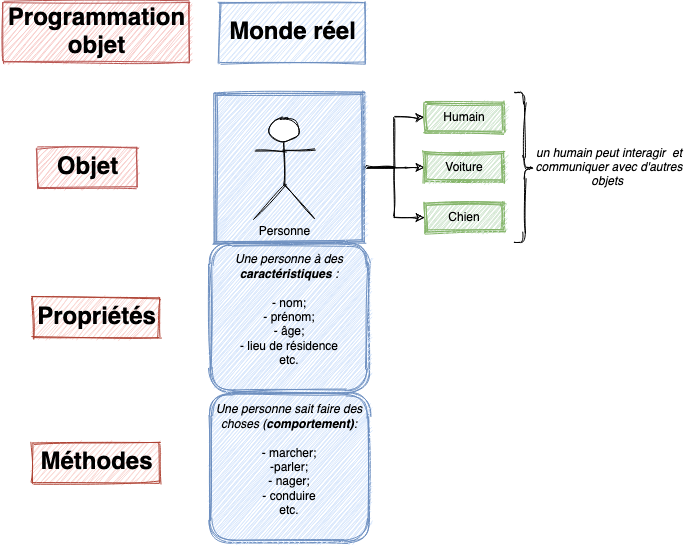
\includegraphics[width=11cm]{images_partie_3/concept_POO.png}}}
    \caption{Le concept d'humain peut-être représenté sous la forme d'un objet \textcopyright L. Terriel, 2020, Diagrams.net}
    \label{fig:concept_POO}
\end{figure}
\newpage
Un objet peut relever d'une même catégorie. Ainsi une voiture est une sorte d'objet avec des caractéristiques et des méthodes propres pouvant appartenir à la catégorie moyen de transport. Celle-ci peut être modélisée au moyen d'une classe en langage orienté objet. La classe est apparentée à une usine qui va créer des objets héritant des propriétés de ces. L'exemple de code ci-dessous montre le moyen de créer un objet \inquote{Personne} en Python :

\lstset{language=Python}
\begin{lstlisting}
"""On définit une classe"""
class Personne:
    def __init__(self, nom, prenom, age, lieu):
        """Le constructeur permet de placer les propriétés de l'objet"""
        self.nom = nom
        self.prenom = prenom
        self.age = age
        self.lieu_de_naissance = lieu
        # propriétés spécifiques pour les actions de l'objet
        self.nombre_de_pas = 0

    """On donne des comportements aux objets (méthodes)"""
    def marcher_en_avant(self):
        self.nombre_de_pas =+ 1
        return print(f'{self.prenom} {self.nom} a fait {self.nombre_de_pas} pas !')
    def parler(self, mot):
        return print(f'mon mot est : \"{mot}\"')

"""On créé un objet Personne (instanciation de l'objet dans la classe Personne)"""
Personne_1 = Personne("Mabillon", "Jean", 388, "Saint-Pierremont")

"""On peut vérifier l'objet créé"""
print(Personne_1)
# >>> <__main__.Personne object at 0x1013862d0>

"""On peut récupérer des propriétés de l'objet"""
print(Personne_1.prenom)
# >>> Jean

"""On peut faire agir l'objet"""
Personne_1.marcher_en_avant()
# >>> Jean Mabillon a fait 1 pas !
Personne_1.parler('De re diplomatica')
# >>> mon mot est : "De re diplomatica"
\end{lstlisting}

C'est cette technique de programmation que nous avons mis en pratique afin de créer les deux modules \citecode{SynSemTS.py} et \citecode{STSig.py}. Nous aurons l'occasion de revenir sur ce dernier module d'expérimentation créé pour tester de nouvelles métriques et qui est encore en phase de développement, dans la section \ref{inter_fonc}.\\

Le diagramme présenté en figure \ref{fig:diag_synsem} montre les différentes classes du module 
\citecode{SynSemTS.py}.

\begin{figure}[h!]
    \centering
    \centerline{\fbox{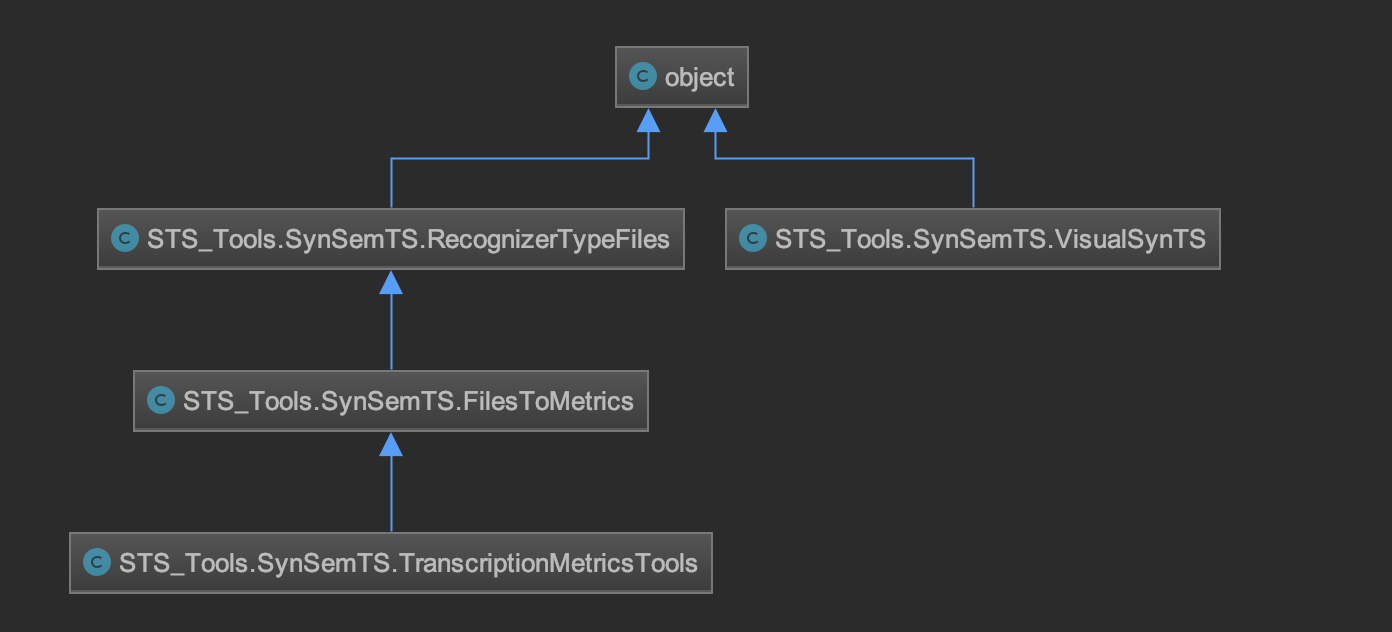
\includegraphics[width=14cm]{images_partie_3/uml_synsemts.png}}}
    \caption{Diagramme du module \citecode{SynSemTS.py} présentant les différentes classes \textcopyright L. Terriel, 2020, \textit{Pycharm}}
    \label{fig:diag_synsem}
\end{figure}

En reprenant le diagramme, une première classe (\citecode{RecognizerTypeFiles}) permet d'identifier les différents types de fichiers correspondant à la transcription vérité terrain, à la prédiction, à l'image et permet également d'effectuer certains traitements textuels sur les fichiers texte, comme le découpage en mots et en caractères. 

Une seconde classe (\citecode{FilesToMetrics}) qui hérite des propriétés et méthodes de la première, effectue la transition entre la première classe et la troisième, en réalisant les calculs de la distance de Levenshtein et récupérant les résultats sous forme d'entier et de matrice. Ce résultat permet en outre, d'effectuer les futurs calculs.

Une troisième classe (\citecode{TranscriptionMetricsTools}), la plus importante, hérite de la première et de la deuxième. Elle se charge de tous les calculs permettant de retrouver les métriques qui seront affichées dans le navigateur \textit{web} (distance de Hamming, WER, CER, indice de Jaccard et similarité cosinus). Dès lors, les objets créés à la fin du script principal \citecode{kraken\_benchmark.py} le sont à partir de la dernière classe. 

Une autre classe est créé indépendamment (\citecode{VisualSynTS}) elle permet de réaliser des objets spécifiques correspondant aux visualisations graphiques affichées dans le navigateur \textit{web}. En revanche, pour des raisons de temps de chargement trop longs, j'ai décidé de créer ces objets dans les routes (\citecode{routing.py}) au moment où l'utilisateur formule une requête pour les consulter.\\

Pour conclure, il n'était pas obligatoire de programmer avec ce paradigme, mais les avantages de la programmation orientée objet sont nombreux et ont séduit pour la suite du projet. 

Chaque objet présente une documentation claire quant à ses propriétés et ses méthodes, ce qui permet de savoir quels types de fonctions on manipule pendant le développement. Les types d'objets créés peuvent servir de base pour d'autres objets (on évite ainsi de réécrire du code existant). On peut réutiliser ces objets dans le cadre d'autres projets en réutilisant certains briques déjà posées. 

Enfin en plus d'obtenir un code plus compréhensible, il est plus facile de le maintenir et de le faire évoluer. On pourra modifier les objets, par exemple ajouter de nouvelles métriques ou les corriger, sans toucher à l'ensemble de l'interface comme la séquence HTR ou la partie affichage dans le navigateur.

\subsubsection{Retour sur les principales difficultés rencontrées}

Parmi les difficultés auxquelles nous nous sommes heurté au cours du développement de l'application, j'ai relevé les points suivants :

\begin{itemize}
    \item La gestion des données d'entrée (fichiers texte, images et modèle) n'est pas encore optimale. Actuellement, l'utilisateur doit stocker ses fichiers à la racine du script principal suivant un système d'étiquetage comme vu plus haut. Ce système pourrait être amélioré;
    \item Durant le développement de la fonction coïncidant avec la séquence HTR, je devais trouver le moyen de stocker et d'associer les fichiers entre-eux sans perdre l'ordre des fichiers pour ne pas mélanger une prédiction avec sa vérité terrain et son image. Je pouvais aboutir à des structures de données (liste de tuples contenant des listes) très complexes à manipuler en raison de leurs longueurs. Je devais souvent lancer le programme en entier, plusieurs fois, pour être sûr que l'ordre n'avait pas été modifié. La programmation objet m'a permis de résoudre le problème;
    \item N'étant pas familier de la programmation objet au moment de coder l'application, beaucoup d'essais on étaient nécessaires pour aboutir au résultat actuel. Le module \citecode{SynSemTS.py} doit encore pouvoir être simplifié. Une réflexion doit être menée sur cet aspect, ce qui permettrait d'accélérer davantage le processus de création des objets à la fin du script principal;
    \item Je n'ai pas réussi à trouver le moyen d'afficher deux visualisations graphiques différentes sur la même route URL. 
\end{itemize}

\section{Suivi sur la conception et retour sur les usages de \textit{Kraken-Benchmark}}

\subsection{La gestion du projet \textit{Kraken-Benchmark}}

Durant le développement de l'application, un ensemble de rituels ont été mis en place afin de s'assurer des retours réguliers lors du développement de l'application.\\

\textbf{Revue de code et intégration continue - }Dans un premier temps, afin de vérifier que le code répondait aux exigences des règles d'usages propres au langage Python (obtenir un code \inquote{pythonique}), et qu'il était suffisamment compréhensible, un système d'intégration continue a été mis en place sur la plate-forme \textit{GitLab} par Alix Chagué au moment de mon arrivée\footnote{Dans le cadre de mon stage il s'agissait du logiciel \textit{Jenkins} interfacé avec la plate-forme Gitlab.}. À chaque fois que j'ajoutai une fonctionnalité ou que j'effectuai une modification dans mon code, je déposais mon code sur \textit{GitLab} par l'intermédiaire du système de versions \textit{Git} : un système de message indique quelles modifications j'avais effectué (\textit{commits}) et le code est envoyé sur la plate-forme (\textit{push}).\\

Au moment où la plate-forme Gitlab recevait mon code, le système d'intégration continue exécutait automatiquement un fichier BASH (\citecode{ci-test.sh}\footnote{Ce fichier est disponible dans les Annexes C}), rédigé par Alix Chagué. 

Ce fichier réalisait un test sur le code source, par le biais du logiciel \textit{Pylint}, pour effectuer une vérification de qualité. \textit{Pylint} utilise les recommandations officielles de la PEP8\footnote{PEP (\textit{Python Enhancement Proposal}), sont connues au sein de la communauté Python pour être des propositions d'améliorations du langage Python qui portent toutes un numéro. La PEP8 peut être vue comme un guide pour rédiger en langage Python et a pour objectif de définir des règles de développement communes entre développeurs : vérifier les indentations du code, les noms de variables, les espaces ou les lignes trop longues; PEP8, URL : \url{https://www.python.org/dev/peps/pep-0008/}} pour s'assurer que les règles de rédaction du code sont respectées. Si le score était supérieur à 7, le système me renvoyait un message de succès. Ma tutrice, en la personne d'Alix Chagué, pouvait alors entreprendre une revue \inquote{manuelle} du code (\textit{code review}) et se concentrer sur ses aspects fonctionnels, une fois que j'avais effectué des propositions de modifications (\textit{Merge Requests}). Dans le cas contraire, je devais reprendre mon code et repasser les tests. 

Ce système, bien qu'en apparence contraignant, m'a obligé à assurer une rigueur pendant la rédaction de mon code, au fur et à mesure des développement et m'a permis d'accroître mes réflexes tels que la rédaction d'une documentation pour chaque fonctions, nommage des variables etc.
\newpage
\textbf{Tests fonctionnels et retours utilisateurs - } Sur ce point, les tests fonctionnels ont primés sur la rédaction de tests unitaires. On entend par tests unitaires un ensemble de scripts rédigés en  langage Python, qui permettent de tester et de s'assurer du bon fonctionnement de plusieurs parties spécifiques du code. Il s'agit d'un choix critiquable mais qui se défend par plusieurs facteurs pouvant expliquer ce manque : \textit{Kraken-Benchmark} est considéré comme une application \inquote{non-critique} et qui fait une large part à l'expérimentation ; elle est actuellement utilisée par un nombre restreint de personnes au sein d'ALMAnaCH ; une fonctionnalité défaillante n'entraîne pas de retard conséquent pour l'avancement du projet, contrairement à une application eScriptorium, par exemple, qui doit être opérationnelle pour un grand nombres d'usages. 

De plus, les difficultés rencontrées pour développer certaines fonctionnalités essentielles de l'application, conjuguées au besoin de pouvoir effectuer des tests sur des données Lectaurep avant la fin du stage, m'a obligé à me concentrer sur l'aspect général et les résultats visibles de l'application, plutôt que de couvrir, par la rédaction de tests longs, chaque détails de fonctionnement.\\

Cependant, si l'outil doit évoluer dans la suite du projet, ou inclure de nouvelles fonctionnalités et hypothétiquement être mis en production à plus grande échelle, la rédaction de tests unitaires s'avérera être une priorité absolue afin s'assurer des bases plus solides.\\

Afin de m'assurer que l'application fonctionnait à chaque modification importante, je l'ai relancé avec mon set de test (dossier \citecode{jules\_verne\_set\_test}) m'assurant ainsi que le code fonctionnait toujours et qu'aucun conflit majeur n'était apparu.\\

Enfin j'ai créé une zone de test, sous la forme d'un rapport d'erreurs (\textit{issue}) sur GitLab pour recueillir les témoignages d'autres utilisateurs. Ainsi Florianne Chiffoleau, ingénieure en recherche et développement au laboratoire  ALMAnaCH, a eu l'occasion de tester les performances de ses modèles de transcription dans \textit{Kraken-Benchmark} afin de de pouvoir les départager, dans le cadre du projet DAHN/MESRI traitant de la correspondance de Paul d'Estournelles de Constant (1852-1924).\\

Ces retours positifs montrent que l'utilisation de l'application peut être généralisée à d'autres projets d'HTR que Lectaurep.\\
\newpage
\subsection{Un tour d'horizon de l'interface \textit{Kraken-Benchmark} et des fonctionnalités actuelles}\label{inter_fonc}
Nous proposons dans cette section de passer en revue les fonctionnalités implémentées actuellement dans Lectaurep et la manière dont on peut interpréter les résultats.

\textbf{La page d'accueil : tableau général de métriques et visualisation par images (Figure \ref{fig:accueil_KB_1} et Figure \ref{fig:accueil_KB_2}) - } La page d'accueil est la première page rencontrée par l'utilisateur. Un tableau de métriques (\textit{Dashboard}) lui permet d'obtenir rapidement des scores sur l'ensemble de son corpus (Figure \ref{fig:accueil_KB_1}). Ces métriques ont été présentées en section \ref{metriques}. \\On peut attirer l'attention sur la distance de Hamming, l'indicateur qui permet de révéler rapidement à l'utilisateur si la taille de la vérité terrain et de la prédiction sont égales. Dans le cas contraire, un symbole \inquote{$\emptyset$} l'indiquera. Un code couleur renseigne les meilleurs scores obtenus (vert) et les scores moins bons (rouge). De plus, des hyperliens placés sur les numéros des images permettent d'accéder à l'image en question avec un niveau plus important de détails \ref{fig:accueil_KB_2}). 
A l'échelle de l'image, certaines métriques du tableau sont répétées afin d'éviter des alternances à l'utilisateur entre le haut et le bas de la page.\\ Un premier graphique montre le nombre de caractères exactement reconnus, supprimés et insérés. Enfin, il est possible d'accéder aux autres fonctionnalités de l'application qui montrent d'autres vues l'image.

\begin{figure}[h!]
    \centering
    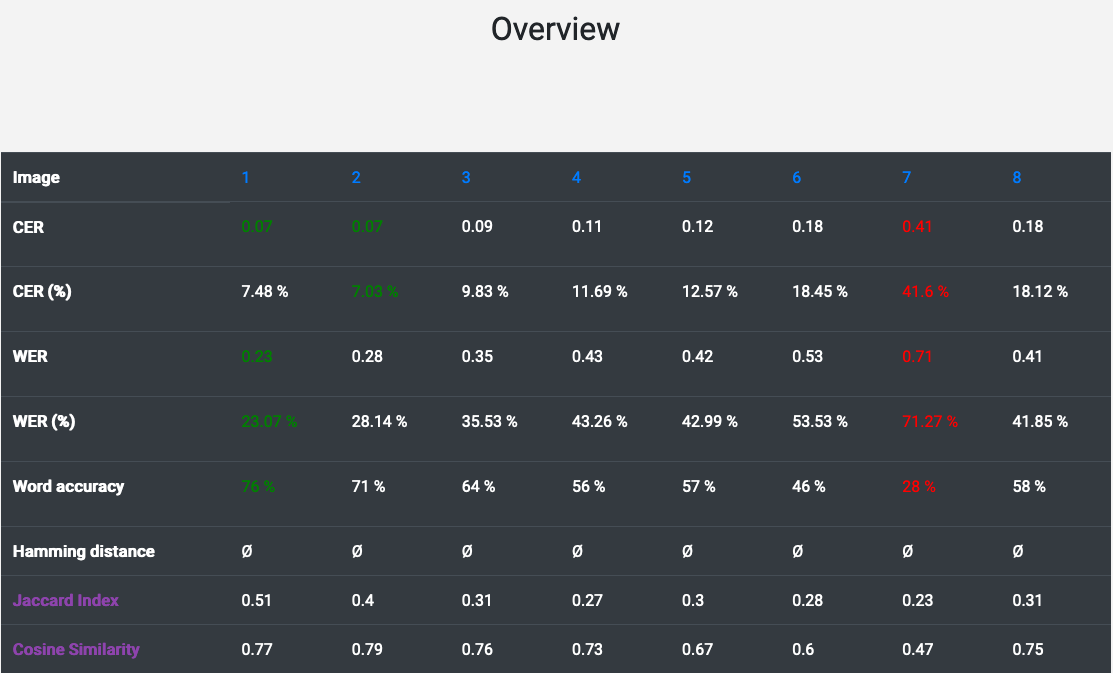
\includegraphics[width=16cm]{images_partie_3/interface_KB/KB_2.png}
        \caption{La page d'accueil : tableau de métriques \textcopyright L.TERRIEL, 2020, \textit{Kraken-Benchmark}}
        \label{fig:accueil_KB_1}
\end{figure}
\begin{figure}[h!]
    \centering
    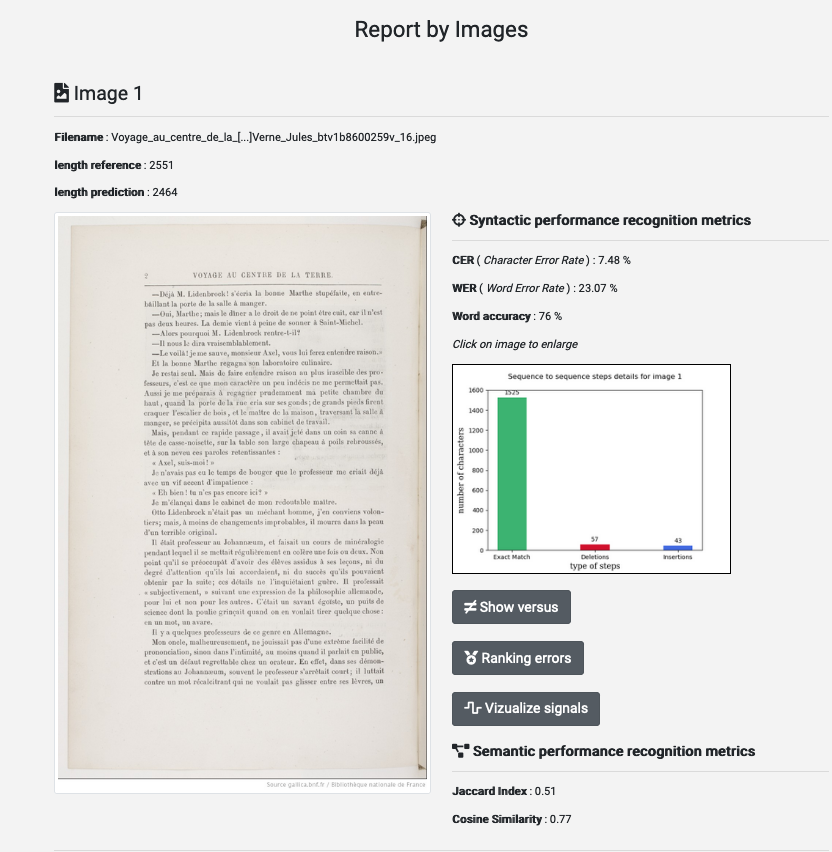
\includegraphics[width=18cm]{images_partie_3/interface_KB/KB_4.png}
        \caption{La page d'accueil : l'image et le graphique des opérations \textcopyright L.TERRIEL, 2020, \textit{Kraken-Benchmark}}
        \label{fig:accueil_KB_2}
\end{figure}
\newpage
\textbf{Une option pour confronter la vérité terrain et la prédiction HTR (Figure \ref{fig:accueil_KB_3}) - } La fonctionnalité \textit{Show versus} de la page d'accueil permet de confronter la vérité terrain dans la colonne de gauche à la prédiction située dans la colonne de droite. La colonne du milieu est une superposition des deux textes. Un code couleur signale à l'utilisateur les caractères parfaitement reconnus en vert, les caractères supprimés ou substitués en rouge, et les insertions en bleu. \\ Au niveau supérieur, la distance de Levensthein indique à l'utilisateur la mesure des différences entre les deux textes, si le score est supérieur à 10, il s'affiche en rouge pour indiquer que le texte contient un grand nombre d'erreurs.
\begin{figure}[h!]
    \centering
    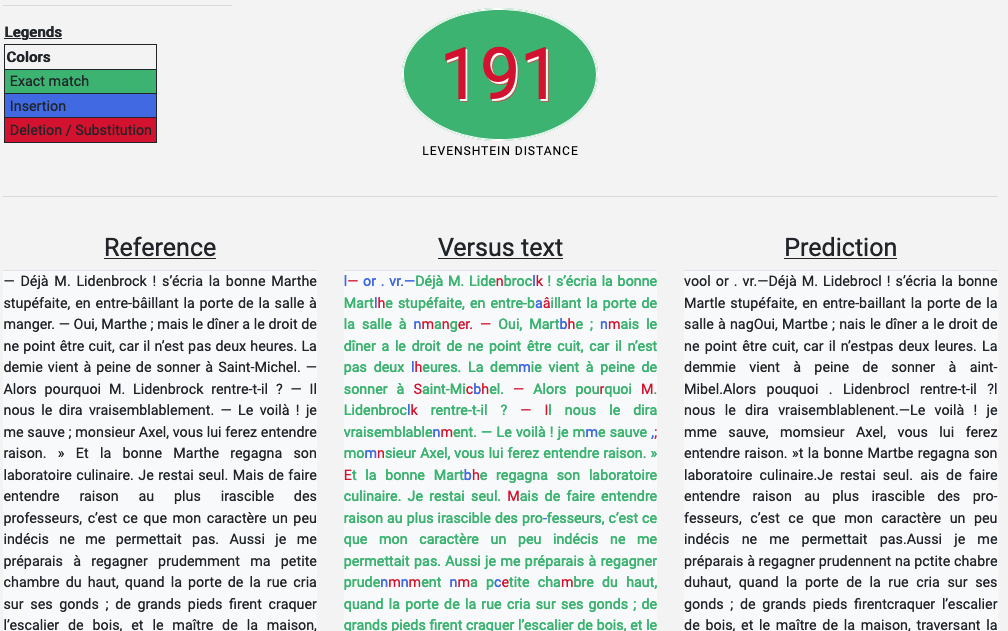
\includegraphics[width=16cm]{images_partie_3/interface_KB/KB_5_VS.png}
        \caption{La fonctionnalité \textit{Show versus} \textcopyright L.TERRIEL, 2020, \textit{Kraken-Benchmark}}
        \label{fig:accueil_KB_3}
\end{figure}
\bigskip

\textbf{Un classement des erreurs les plus fréquentes (Figure \ref{fig:accueil_KB_4}) - }  La fonctionnalité \textit{Ranking errors} est un classement des erreurs les plus fréquentes réalisé par le modèle sur l'image. L'utilisateur dispose d'une indication sur la fréquence d'apparition de l'erreur et des détails sur le caractère de la vérité terrain qui a été confondu par le modèle. L'absence de caractère indique un \inquote{espace}. Sur la droite, l'utilisateur dispose d'une autre vue sous la forme d'une \inquote{matrice de confusion}. Il ne s'agit pas d'une \inquote{matrice de confusion} au sens strict, c'est-à-dire une classification des données par classes, il s'agit du même classement des paires d'erreurs mais seulement pour les dix erreurs les plus fréquentes (sinon la matrice devient illisible). 

Ainsi en ordonnée sont disposés les caractères du texte de référence et en abscisses les caractères de la phrase prédite. L'alignement d'un caractère $x$ et d'un caractère $y$ nous donne la fréquence de la confusion. Le classement détaillé à gauche et la matrice à droite, sont équivalentes. 
\newpage
\begin{figure}[h!]
    \centering
    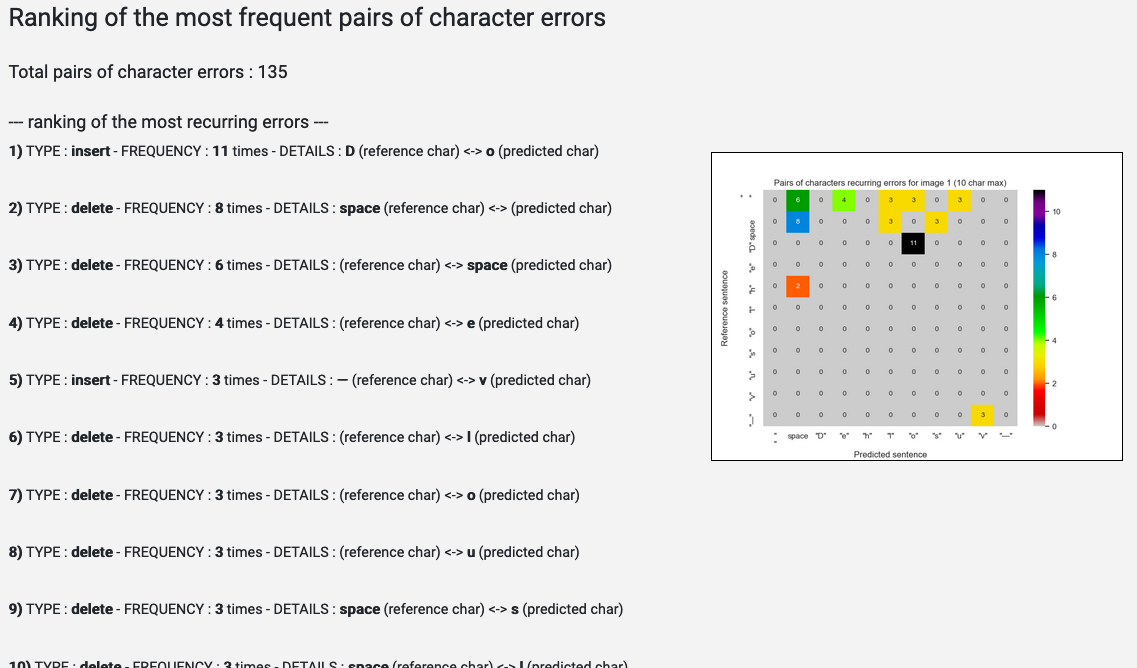
\includegraphics[width=15cm]{images_partie_3/interface_KB/KB_6_rank.png}
        \caption{La fonctionnalité \textit{Ranking errors} \textcopyright L.TERRIEL, 2020, \textit{Kraken-Benchmark}}
        \label{fig:accueil_KB_4}
\end{figure}
\bigskip

\textbf{Une visualisation des phrases sous la forme de signaux (Figures \ref{fig:accueil_KB_5} et \ref{fig:accueil_KB_6}) - } La fonctionnalité \textit{Vizualize signals} permet de générer une visualisation expérimentale qui appartient au module \citecode{STSig.py}\footnote{Le détail de l'algorithme est présenté dans le \textit{notebook} Jupyter intitulé \inquote{Evaluation de la similarité entre deux séquences dans le contexte de la reconnaissance automatique de caractères}.}. 

J'ai essayé de superposer sous la forme de droites passant par des points dont les coordonnées correspondent, en abscisses, aux séquences de caractères, et, en ordonnée, des valeurs numériques correspondant aux caractères eux-mêmes accessibles par le biais de l'onglet \textit{Dictionnary position-weight characters}. Il s'agit d'un dictionnaire qui permet de décoder les valeurs numériques de l'axe des ordonnées. 

Ces valeurs sont attribuées comme suit : un caractère de ponctuation sera associé à une valeur de 0.5, un espace à 0, et un caractère non reconnu ou des valeurs numéraires à -1.

Chaque caractères de l'alphabet latin est encodé de la manière suivante : \inquote{a} vaudra 1, \inquote{b} vaudra 2, \inquote{c} vaudra 3 etc. Si ces caractères subissent une ou des transformation(s) on leur ajoute un poids : une accentuation vaudra 0.5, une capitalisation 0.1 et une capitalisation plus une accentuation 0.6 par exemple si \inquote{a} vaut 1 alors \inquote{à} vaudra 1.5 et un \inquote{À} vaudra 1.6 de même si \inquote{b} vaut 2 alors \inquote{B} vaudra 2.1 etc. Dès lors, l'algorithme encode la vérité terrain et la prédiction selon ce système de valeurs numériques et les deux textes sont superposés dans le graphiques selon ce système de coordonnées. Afin d'interpréter les résultats, si un caractère de la prédiction diffère du caractère de la référence un système de boîtes d'erreurs (\textit{error boxes}) se met en place sur les points représentants les caractères de la prédiction divergeant de la référence. On peut alors interpréter certains phénomènes sur le graphique pour comprendre les erreurs survenues et récurrentes (Cf. Figure \ref{fig:accueil_KB_7}). Pour ne pas surcharger le graphique et le rendre illisible, un système d'intervalles est réglable (Cf. Figure \ref{fig:accueil_KB_6}) par l'utilisateur pour accéder à certaines parties du texte par le biais de l'onglet \textit{Settings sequence signals}. Cette représentation est un essai, et elle ne peut se substituer aux métriques classiques d'évaluation des modèles HTR présentées plus haut; de plus un trop grand nombre d'erreurs rend rapidement la lecture impossible.
\begin{figure}[h!]
    \centering
    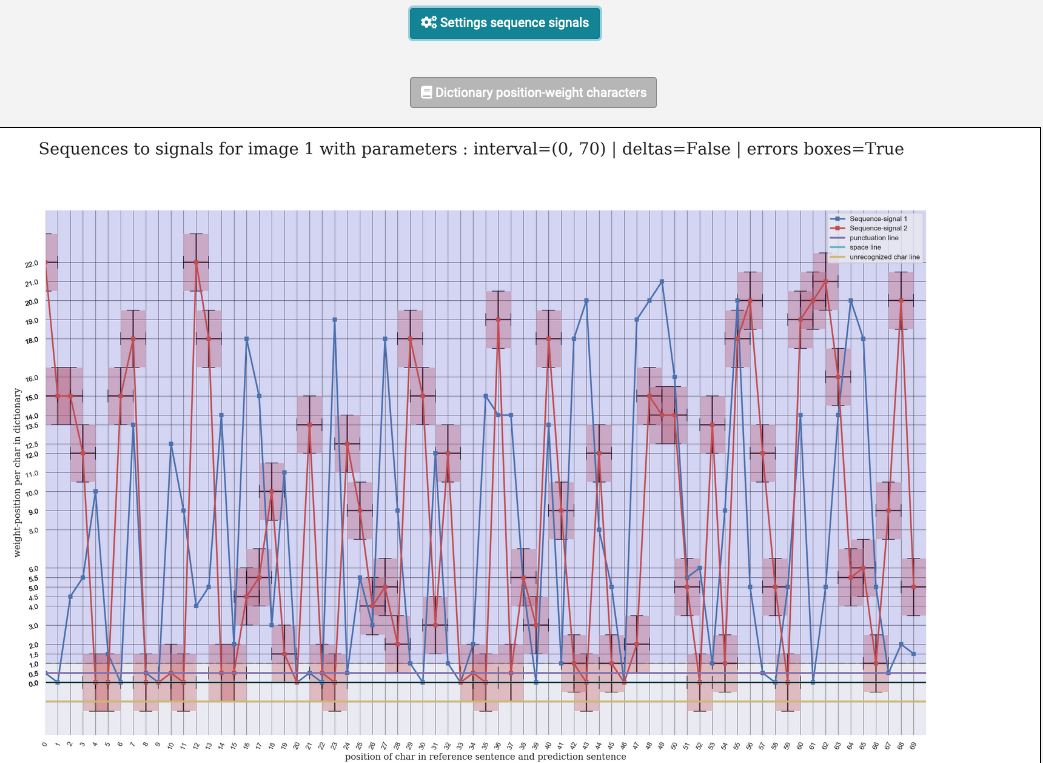
\includegraphics[width=18cm]{images_partie_3/interface_KB/KB_7_STS.png}
        \caption{La fonctionnalité \textit{Vizualize signals} \textcopyright L.TERRIEL, 2020, \textit{Kraken-Benchmark}}
        \label{fig:accueil_KB_5}
\end{figure}
\begin{figure}[h]
    \centering
    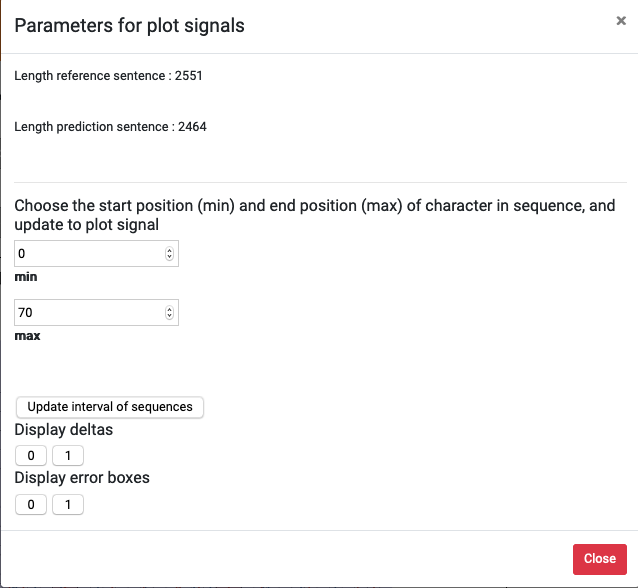
\includegraphics[width=10cm]{images_partie_3/interface_KB/KB_8_STS.png}
        \caption{La fenêtre \inquote{pop-up} qui permet de régler l'intervalle des séquences à visualiser dans le graphique de \textit{Vizualize signals} \textcopyright L.TERRIEL, 2020, \textit{Kraken-Benchmark}}
        \label{fig:accueil_KB_6}
\end{figure}
\begin{figure}[h]
    \centering
    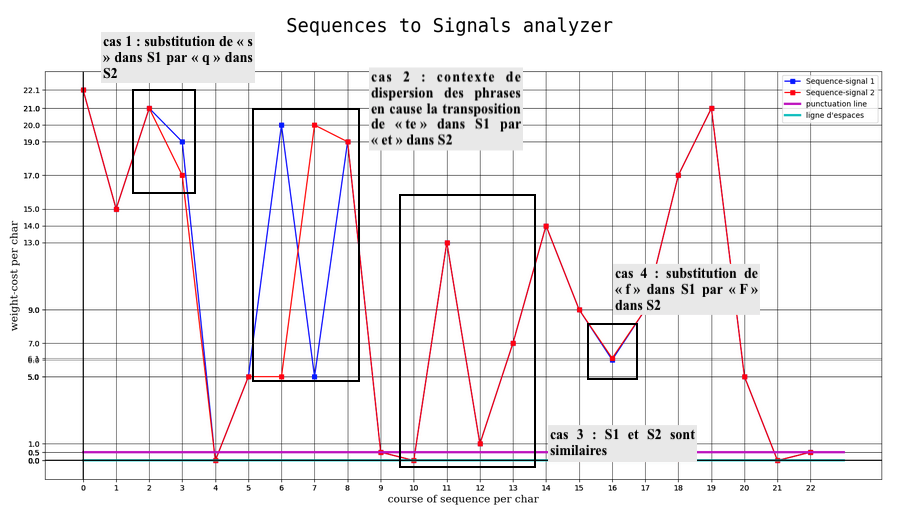
\includegraphics[width=18cm]{images_partie_3/interface_KB/graph_sequence_signal.png}
        \caption{Exemples d'interprétations de la fonctionnalité  \textit{Vizualize signals}\textcopyright L.TERRIEL, 2020, \textit{Kraken-Benchmark}}
        \label{fig:accueil_KB_7}
\end{figure}

\newpage
\section{Perspectives d'amélioration techniques pour l'application}\label{perspectives_amélios}

Dans la section \ref{objectifs}, nous avions fixés un certains nombres d'objectifs à atteindre. A la fin du stage, un certains nombres de ces tâches ont été réalisé. L'outil proposé actuellement est opérationnel pour tester des modèles HTR. Cependant, l'outil peut encore être largement amélioré :
\begin{itemize}
    \item Da
\end{itemize}



\chapter{Tests de Kraken-Benchmark sur les images de répertoires de notaires}\label{tests_KB_lectaurep}
\section{Préparation du corpus et mise en place des tests}
mettre les images de problèmes et pas les répertoires entiers 
- regrouper particularisme d'écriture 
- regrouper difficultés matériels 

\section{Déroulement et résultats des tests}

radars 


\section{Les premiers résultats, un bilan mitigé ?}



Les ré
reprendre mémoire alix sur les objectifs  CER et WER Transkribus + MLB pp. 7 avec références

-> Les modèles utilisés présenté des problèmes sous entrainement et sur entrainement



Globalement les problèmes sur des données plus nombreuses et mixtes. Initialement le random set (700) devait être entièrement trasncrits 
pour permettre des entrainements sur des variétés de répertoire nombreux et entrainer un modèle général. Ce qui permettra d'atteindre des accuracy plus intéréssants et finetuner des modèles pour certains types de notaires. 
la variabilité des écritures obstacle dans la reconnaissance ex. ecritures très sérrés
Cependant l'approche actuel du DMC consiste à transcrire notaire par notaire (Riant, puis Dufour Marotte), pour des questions de facilité pour les annotateurs du projet LEctaurep, à partir du golden set. Conséquences : 1) fournis des données centrés sur un notaire et 2) pas assez nombreuses 3) rend compte de résultats toujours très faibles. 

=> Alix a entrainé récémment deux modèles qui pourront être tester sur qui expose ces difficultés (graphiques Alix et résultats) mais ces nouveaux modèles n'ont pas encore testés dans KBapp

=> il faut donc attendre encore un plus grands nombres d'annotations pour exploiter ce random set et fournir des données plus nombreuses et variés. 

Cependant vieux modèles


La plateforme peut déjà servir de pour les futures tests pour lorsque les premiers modèles de transcription